% Options for packages loaded elsewhere
\PassOptionsToPackage{unicode}{hyperref}
\PassOptionsToPackage{hyphens}{url}
\PassOptionsToPackage{dvipsnames,svgnames,x11names}{xcolor}
%

\documentclass[]{cik}%%%%where rsos is the template name

\usepackage{amsmath,amssymb}
\usepackage{lmodern}
\usepackage{iftex}
\ifPDFTeX
  \usepackage[T1]{fontenc}
  \usepackage[utf8]{inputenc}
  \usepackage{textcomp} % provide euro and other symbols
\else % if luatex or xetex
  \usepackage{unicode-math}
  \defaultfontfeatures{Scale=MatchLowercase}
  \defaultfontfeatures[\rmfamily]{Ligatures=TeX,Scale=1}
\fi
% Use upquote if available, for straight quotes in verbatim environments
\IfFileExists{upquote.sty}{\usepackage{upquote}}{}
\IfFileExists{microtype.sty}{% use microtype if available
  \usepackage[]{microtype}
  \UseMicrotypeSet[protrusion]{basicmath} % disable protrusion for tt fonts
}{}
\makeatletter
\@ifundefined{KOMAClassName}{% if non-KOMA class
  \IfFileExists{parskip.sty}{%
    \usepackage{parskip}
  }{% else
    \setlength{\parindent}{0pt}
    \setlength{\parskip}{6pt plus 2pt minus 1pt}}
}{% if KOMA class
  \KOMAoptions{parskip=half}}
\makeatother
\usepackage{xcolor}
\setlength{\emergencystretch}{3em} % prevent overfull lines
\setcounter{secnumdepth}{-\maxdimen} % remove section numbering
% Make \paragraph and \subparagraph free-standing
\ifx\paragraph\undefined\else
  \let\oldparagraph\paragraph
  \renewcommand{\paragraph}[1]{\oldparagraph{#1}\mbox{}}
\fi
\ifx\subparagraph\undefined\else
  \let\oldsubparagraph\subparagraph
  \renewcommand{\subparagraph}[1]{\oldsubparagraph{#1}\mbox{}}
\fi


\newlength{\cslhangindent}
\setlength{\cslhangindent}{1.5em}
\newlength{\csllabelwidth}
\setlength{\csllabelwidth}{3em}
\newlength{\cslentryspacingunit} % times entry-spacing
\setlength{\cslentryspacingunit}{\parskip}
\newenvironment{CSLReferences}[2] % #1 hanging-ident, #2 entry spacing
 {% don't indent paragraphs
  \setlength{\parindent}{0pt}
  % turn on hanging indent if param 1 is 1
  \ifodd #1
  \let\oldpar\par
  \def\par{\hangindent=\cslhangindent\oldpar}
  \fi
  % set entry spacing
  \setlength{\parskip}{#2\cslentryspacingunit}
 }%
 {}
\usepackage{calc}
\newcommand{\CSLBlock}[1]{#1\hfill\break}
\newcommand{\CSLLeftMargin}[1]{\parbox[t]{\csllabelwidth}{#1}}
\newcommand{\CSLRightInline}[1]{\parbox[t]{\linewidth - \csllabelwidth}{#1}\break}
\newcommand{\CSLIndent}[1]{\hspace{\cslhangindent}#1}

\usepackage{booktabs}
\usepackage{longtable}
\usepackage{array}
\usepackage{multirow}
\usepackage{wrapfig}
\usepackage{float}
\usepackage{colortbl}
\usepackage{pdflscape}
\usepackage{tabu}
\usepackage{threeparttable}
\usepackage{threeparttablex}
\usepackage[normalem]{ulem}
\usepackage{makecell}
\usepackage{xcolor}
\usepackage{orcidlink}
\definecolor{mypink}{RGB}{219, 48, 122}
\makeatletter
\makeatother
\makeatletter
\makeatother
\makeatletter
\@ifpackageloaded{caption}{}{\usepackage{caption}}
\AtBeginDocument{%
\ifdefined\contentsname
  \renewcommand*\contentsname{Table of contents}
\else
  \newcommand\contentsname{Table of contents}
\fi
\ifdefined\listfigurename
  \renewcommand*\listfigurename{List of Figures}
\else
  \newcommand\listfigurename{List of Figures}
\fi
\ifdefined\listtablename
  \renewcommand*\listtablename{List of Tables}
\else
  \newcommand\listtablename{List of Tables}
\fi
\ifdefined\figurename
  \renewcommand*\figurename{Figure}
\else
  \newcommand\figurename{Figure}
\fi
\ifdefined\tablename
  \renewcommand*\tablename{Table}
\else
  \newcommand\tablename{Table}
\fi
}
\@ifpackageloaded{float}{}{\usepackage{float}}
\floatstyle{ruled}
\@ifundefined{c@chapter}{\newfloat{codelisting}{h}{lop}}{\newfloat{codelisting}{h}{lop}[chapter]}
\floatname{codelisting}{Listing}
\newcommand*\listoflistings{\listof{codelisting}{List of Listings}}
\makeatother
\makeatletter
\@ifpackageloaded{caption}{}{\usepackage{caption}}
\@ifpackageloaded{subcaption}{}{\usepackage{subcaption}}
\makeatother
\makeatletter
\@ifpackageloaded{tcolorbox}{}{\usepackage[many]{tcolorbox}}
\makeatother
\makeatletter
\@ifundefined{shadecolor}{\definecolor{shadecolor}{rgb}{.97, .97, .97}}
\makeatother
\makeatletter
\makeatother
\ifLuaTeX
  \usepackage{selnolig}  % disable illegal ligatures
\fi
\IfFileExists{bookmark.sty}{\usepackage{bookmark}}{\usepackage{hyperref}}
\IfFileExists{xurl.sty}{\usepackage{xurl}}{} % add URL line breaks if available
\urlstyle{same} % disable monospaced font for URLs
\hypersetup{
  pdftitle={Investigating Imperceptible Vibrotactile Stimulation during a Force Stability Task},
  pdfauthor={Courtney A. Haynes; Matthew S. Tenan; Antony D. Passaro; Andrew J. Tweedell},
  pdfkeywords={key1, key2, key3},
  colorlinks=true,
  linkcolor={blue},
  filecolor={Maroon},
  citecolor={Blue},
  urlcolor={blue},
  pdfcreator={LaTeX via pandoc}}


\usepackage{authblk}
\begin{document}
\captionsetup[table]{labelformat=empty}
\captionsetup[figure]{labelformat=empty}
\raggedbottom

%%%% Article title to be placed here
\title{Investigating Imperceptible Vibrotactile Stimulation during a
Force Stability Task}


%\author{
%% Courtney A. Haynes\textsuperscript{1},
%% Matthew S. Tenan\textsuperscript{2},
%% Antony D. Passaro\textsuperscript{3},
%% Andrew J. Tweedell\textsuperscript{4}%}

  \author[1,*]
  {Courtney A. Haynes}
  \author[2]
  {Matthew S. Tenan}
  \author[3]
  {Antony D. Passaro}
  \author[1]
  {Andrew J. Tweedell}

\affil[1]{U.S. Combat Capabilities Development Command, Army Research
Laboratory, Aberdeen Proving Ground, MD, USA}
\affil[2]{Optimum Performance Analytics Associates, Apex, NC, USA}
\affil[3]{U.S. Combat Capabilities Development Command, Army Research
Laboratory, ARL West, Playa Vista, CA, USA}

  \corrauthor[*]{fake@fake.edu}

\address{ \\ }
%%%% Subject entries to be placed here %%%%
\subject{
Subject1,
Subject2}

%%%% Keyword entries to be placed here %%%%
\keywords{
key1,
key2,
key3}

%%%% Insert corresponding author and its email address}
%\corres{
%  \\
%{\footnotesize }
%}
\inserttype{
{\Large Research}
}

\insertcite{
  {10.51224/cik.2022.41}
}


\editor{
  Matthieu Boisgontier
}

%%%% Abstract text to be placed here %%%%%%%%%%%%
\begin{abstract}
Imperceptible vibratory noise stimulation has shown to improve stability
for both whole body postural control and simple motor control tasks.
Noise stimulation is theorized to elicit a stochastic resonance-like
effect within the somatosensory system, but there is disagreement in the
literature regarding an optimal stimulation level for motor stability in
humans. To explore vibrotactile stimulation, eighteen (18) participants
performed an isometric finger flexion task with visual feedback while
receiving noise stimulation scaled to varying percentages of their
sub-sensory threshold level. Performance was quantified as the
root-mean-square (RMS) error between the target force and the actual
generated force values. The goals of the study were to determine: 1)
whether force stability is significantly better when receiving their
custom ``principal'' stimulation compared to other sub-sensory
stimulation levels, and 2) if an individual's principal stimulation
level may be predicted by either their maximal voluntary contraction
(MVC) or sub-sensory threshold level. A main effect of noise stimulation
was observed (p \textless{} .001) indicating significantly better
performance (lower RMS error) during the force stability task when
individualized principal noise stimulation was applied. At the group
level, task performance was significantly improved with principal noise
stimulation compared to other stimulation levels (p ≤ .019). At the
individual level, however, performance at the principal stimulation
level was only significantly different than the distribution of errors
for other stimulation levels for two individuals. Moderate to strong
Spearman correlations (rs = .56 and rs = .65, respectively) suggest
principal stimulation level increases with MVC and sub-sensory
threshold.
\end{abstract}
%%%%%%%%%%%%%%%%%%%%%%%%%%%

%% Some pieces required from the pandoc template
\providecommand{\tightlist}{%
  \setlength{\itemsep}{0pt}\setlength{\parskip}{0pt}}
\providecommand{\EndFirstPage}{%
}

\definecolor{jobcolor}{cmyk}{0,0,0,.95}
\definecolor{joblightcolor}{cmyk}{0,0,0,.95}
\definecolor{abstractcolor}{RGB}{207, 250, 209}
\definecolor{copyrightcolor}{RGB}{207, 250, 209}

\maketitle

\newpage\ifdefined\Shaded\renewenvironment{Shaded}{\begin{tcolorbox}[breakable, sharp corners, borderline west={3pt}{0pt}{shadecolor}, boxrule=0pt, enhanced, interior hidden, frame hidden]}{\end{tcolorbox}}\fi

\hypertarget{introduction}{%
\section{Introduction}\label{introduction}}

In recent decades, vibrotactile noise stimulation has received attention
as a possible intervention to improve somatosensory function and
supplement postural control (\protect\hyperlink{ref-Galica2009}{Galica
et al., 2009}; \protect\hyperlink{ref-Lipsitz2015}{Lipsitz et al.,
2015}; \protect\hyperlink{ref-magalhuxe3es2011}{Magalhães \& Kohn,
2010}; \protect\hyperlink{ref-Priplata2002}{A. Priplata et al., 2002}).
Although the mechanism by which this intervention is effective is still
uncertain, it has been theorized that mechanical noise stimulation
elicits a stochastic resonance-like effect on the somatosensory system
(\protect\hyperlink{ref-Collins2003}{Collins et al., 2003};
\protect\hyperlink{ref-Manjarrez2002}{Manjarrez et al., 2002};
\protect\hyperlink{ref-Moss2003}{Moss \& Milton, 2003}). Stochastic
resonance (SR) is a naturally occurring phenomenon in which the
detection of a signal in a non-linear system is improved with the
application of random noise rather than degraded by it
(\protect\hyperlink{ref-benzi1981}{Benzi et al., 1981};
\protect\hyperlink{ref-gammaitoni1998}{Gammaitoni et al., 1998};
\protect\hyperlink{ref-McDonnell2009}{McDonnell \& Abbott, 2009}). Here,
the somatosensory system serves as the non-linear system. The addition
of noise may affect ion permeability of the mechanoreceptors
(\protect\hyperlink{ref-Bezrukov1995}{Bezrukov \& Vodyanoy, 1995}) and
may also sum constructively with the non-linear input signal increasing
the likelihood that any near-threshold signal level will be positively
detected (\protect\hyperlink{ref-McDonnell2009}{McDonnell \& Abbott,
2009}; \protect\hyperlink{ref-Moss2004}{Moss, 2004}). In other words,
the application of vibrotactile noise may sharpen one's control of body
position by providing additional sensory information and increasing the
body's ability to detect and respond to changes in body orientation.
Vibratory noise stimulation has shown to be effective in reducing
postural sway among healthy young subjects as well as elderly subjects
and patients with degraded somatosensory function due to diabetes and
stroke (\protect\hyperlink{ref-Collins2003}{Collins et al., 2003};
\protect\hyperlink{ref-magalhuxe3es2011}{Magalhães \& Kohn, 2010};
\protect\hyperlink{ref-Priplata2002}{A. Priplata et al., 2002};
\protect\hyperlink{ref-Priplata2006}{A. A. Priplata et al., 2005}).
Though positive effects are most often elicited through direct
stimulation of the end effector (e.g.~feet to improve balance), benefits
have also been demonstrated with indirect stimulation. For example,
stimulation of the upper extremity in each of 4 different locations can
improve grasp reaction time to perturbations at the hand
(\protect\hyperlink{ref-Hur2014}{Pilwon Hur et al., 2014}). Others have
demonstrated that stimulation of the upper extremities improves tactile
sensation at the fingers
(\protect\hyperlink{ref-Lakshminarayanan2015}{Lakshminarayanan et al.,
2015}). Magalhães \& Kohn
(\protect\hyperlink{ref-magalhuxe3es2011}{2010}) demonstrated that
stimulation of the fingertip even during instances of light touch for
stance support can reduce postural sway.

Much of the previous work demonstrating the efficacy of vibrotactile
noise stimulation has involved short-duration standing balance trials or
isometric force production with the finger. This implies that the noise
stimulation effect may be observed immediately without requiring a
period of acclimation. While stabilizing effects have been observed for
supra-sensory application of vibratory noise
(\protect\hyperlink{ref-magalhuxe3es2011}{Magalhães \& Kohn, 2010}), at
least one study suggests that supra-sensory applications may have a
destabilizing effect due to the subject's awareness of it
(\protect\hyperlink{ref-Simeonov2011}{Simeonov et al., 2011}). Thus, the
transparency of imperceptible stimulation and the immediacy of its
effects make it an attractive intervention to aid stability rapidly and
without distracting attention or otherwise disturbing the user.

Developing interventions which utilize imperceptible noise stimulation
to aid with postural stability has been of interest for many years
(\protect\hyperlink{ref-Collins2003}{Collins et al., 2003};
\protect\hyperlink{ref-Lipsitz2015}{Lipsitz et al., 2015};
\protect\hyperlink{ref-magalhuxe3es2011}{Magalhães \& Kohn, 2010};
\protect\hyperlink{ref-Priplata2002}{A. Priplata et al., 2002}).
Currently, however, more research is needed regarding the signal content
and amplitude that elicits the greatest benefits. In some cases,
research groups have elicited postural stability improvements by
applying imperceptible vibrotactile noise stimulation as a prescribed
percentage (70-90\%) of an individual's sub-sensory threshold level
(\protect\hyperlink{ref-Galica2009}{Galica et al., 2009};
\protect\hyperlink{ref-Lipsitz2015}{Lipsitz et al., 2015};
\protect\hyperlink{ref-Priplata2002}{A. Priplata et al., 2002}). Other
research has suggested that there exists an optimal stimulation level
which elicits greater performance improvements compared to stimulation
at alternative levels (\protect\hyperlink{ref-Manjarrez2002}{Manjarrez
et al., 2002};
\protect\hyperlink{ref-Mendez-Balbuena2012}{Mendez-Balbuena et al.,
2012}; \protect\hyperlink{ref-Trenado2014}{Trenado et al., 2014}).

We aimed to further explore the prescription of vibrotactile noise
stimulation in a directed motor control task. Participants completed a
series of ramp-and-hold trials in which they attempted to maintain an
isometric finger flexion force. During these trials, participants
received imperceptible white Gaussian vibratory noise (≤ 500 Hz)
stimulation which was scaled to specific percentages of the individual's
sub-sensory threshold level. Task performance was quantified as a
root-mean-square (RMS) error between the target and the generated
isometric force values. The stimulation level which resulted in the best
performance was designated as the individual's principal stimulation
level. Using these results, we aimed to: 1) evaluate at the group and
individual level whether performance with the principal stimulation
level was significantly different than task performance at other
sub-sensory stimulation levels, and 2) determine whether an individual's
principal stimulation level are related to either maximal voluntary
contraction (MVC) force or sub-sensory threshold.

\newpage

\hypertarget{methods}{%
\section{Methods}\label{methods}}

The methods described here were part of a larger study conducted to
explore the varying neurophysiological effects of vibrotactile noise
stimulation during a finger flexion force stability task. As a component
of that study, it was necessary to identify the subthreshold stimulation
level which elicited the best force stability during a ramp-and-hold
finger flexion task.

\hypertarget{participants}{%
\subsection{Participants}\label{participants}}

Eighteen (18) young male subjects with a mean age of 25.8\pm6.2 years
were recruited to participate in this study. Male subjects were
recruited to avoid confounds due to previously reported sex differences
in motor neuron discharge rate (\protect\hyperlink{ref-Peng2018}{Peng et
al., 2018}; \protect\hyperlink{ref-Tenan2016}{Tenan et al., 2015}).
Participants had no history of pain, surgery, or injury to the dominant
upper extremity. Participants were also free from metabolic and
neurological disorders, cardiovascular dysfunction, and did not take
blood thinning medications. All methods were reviewed and approved by
the Institutional Review Board of the U.S. Army Research Laboratory.
Participants provided verbal and written informed consent prior to
participation.

\hypertarget{maximal-voluntary-contraction-mvc-procedures}{%
\subsection{Maximal Voluntary Contraction (MVC)
Procedures}\label{maximal-voluntary-contraction-mvc-procedures}}

Participants were seated at an adjustable height desk equipped with a
custom instrumented grip (Figure~\ref{fig-1}). The height of the desk
was adjusted such that the participant could sit up straight with their
supine forearm resting flat on the surface of the desk. A custom
adjustable cradle was mounted to the edge of the table to secure the
position of the upper arm and standardize arm position between
participants and between trials for the same participant
(Figure~\ref{fig-1} A). The grip consisted of a plastic rod with a
trigger-like mechanism instrumented with a compression load cell
(LCM302-50, Omega Engineering, Inc., Stamford, CT). The angular
orientation of the grip was adjustable to afford a comfortable neutral
position for the wrist while the forearm and hand remained in supine
position. The distance of the grip from the participant was adjusted
such that the middle phalanx of the second finger engaged the trigger
mechanism, and the remaining fingers curled comfortably around the
plastic rod. All finger flexion tasks were completed with the hand and
forearm in this standardized supine position.

\begin{figure}

{\centering 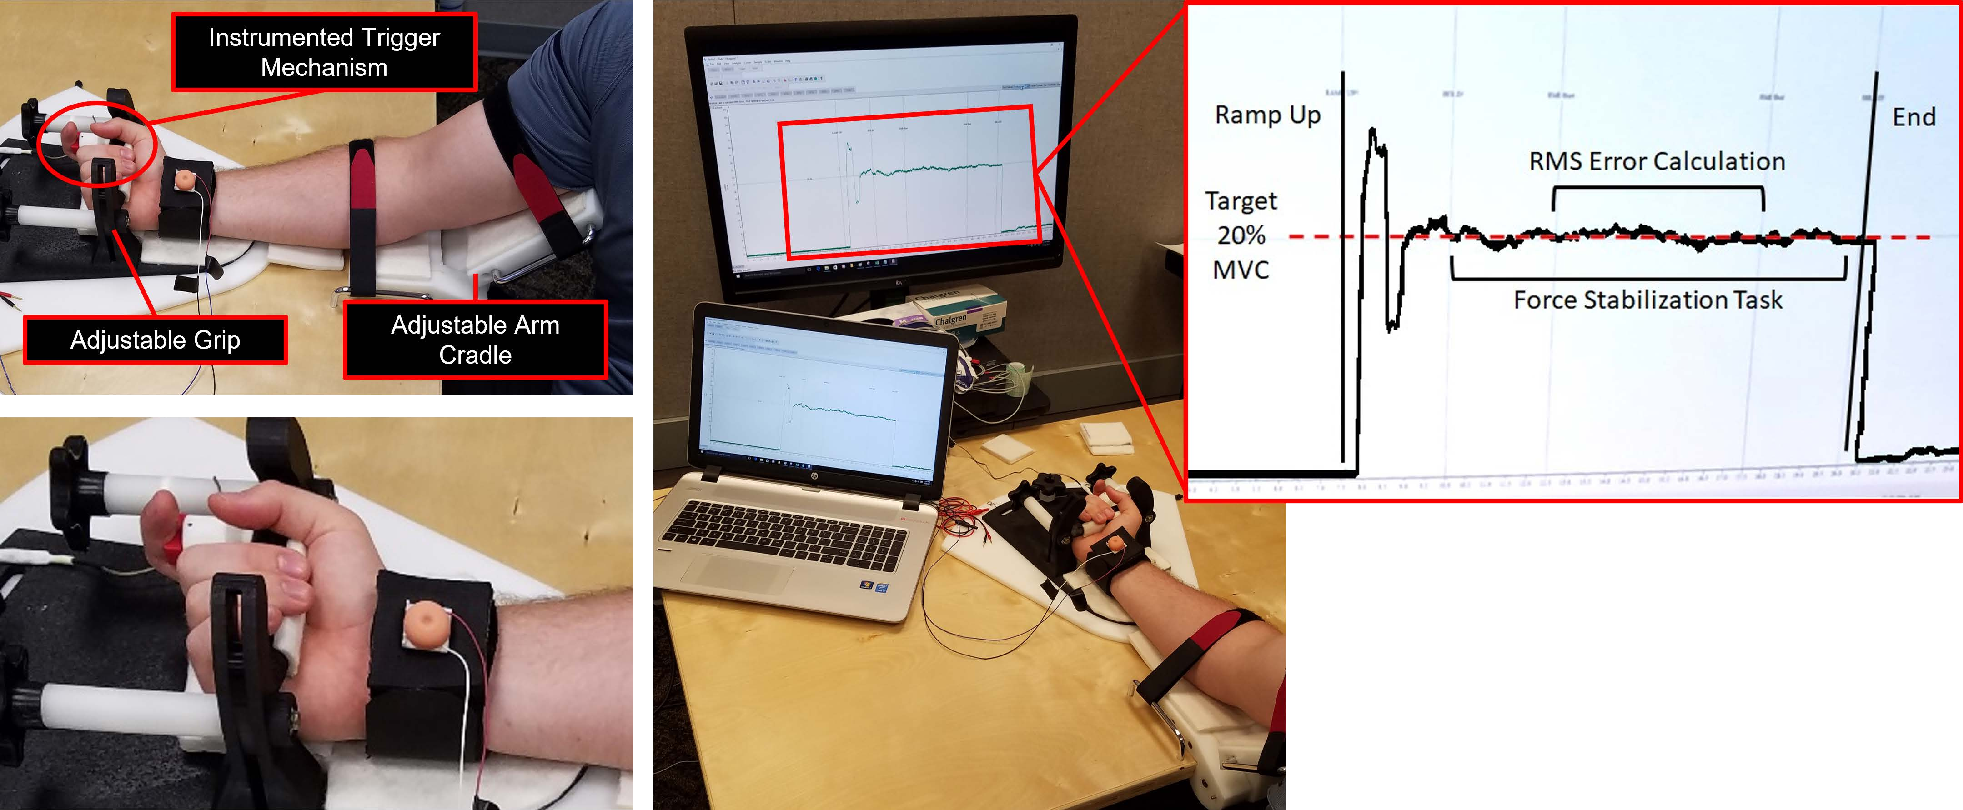
\includegraphics[width=1\textwidth,height=\textheight]{./figures/fig1.pdf}

}

\caption{\label{fig-1}(A) A participant properly positioned and secured
in the adjustable cradle and engaging the trigger-like mechanism. (B) A
close-up image of the trigger mechanism and the vibrotactile stimulator
embedded in a neoprene wrist band. (C) A participant completing the
ramp-and-hold task with visual feedback provided. (D) Magnified and
enhanced image of visual feedback indicating the target 20\% MVC level,
the prompt to apply force and reach target level (`Ramp Up'), the
duration of the force stabilization task, the middle 5 seconds of data
used for the RMS error calculation, and the completion of the trial
(`End').}

\end{figure}

Prior to completing other experimental tasks, participants completed a
series of maximum exertions to determine their maximum finger flexion
force. Participants were instructed to produce force only by squeezing
their pointer finger against the trigger mechanism and were asked to
refrain from flexing their wrist or elbow. A monitor positioned at the
participant's eye level presented visual prompts and force feedback via
custom data acquisition script (Spike2, Cambridge Electronic Design
Ltd., Cambridge, England, UK). Verbal encouragement was also provided
during maximum voluntary contractions (MVCs). MVCs were sustained for 5
seconds each with a rest period of 1 minute between successive attempts.
Force data were amplified using a bridge amplifier (Digitimer NL109,
Digitimer Ltd., Ft. Lauderdale, FL) with a gain of 100 and were recorded
at a rate of 1000 Hz via a Micro 1401-3 data acquisition unit (Cambridge
Electronic Design Limited, Cambridge, England, UK). After three
exertions, the values for each MVC were analyzed. If the three
consecutive MVC values were within 10\% of each other, the highest MVC
was recorded as the maximum force value. If there was more than a 10\%
difference between the highest and lowest recorded MVC attempt, the
participant was given 5 minutes of rest and another round of three MVCs
were completed. This procedure continued until a maximum force value was
identified. For all participants, this was accomplished in three or
fewer rounds of MVC attempts (n=16 for 1 round, n=1 for 2 rounds, n=1
for 3 rounds).

Following the MVC procedures, each participant's individual sub-sensory
threshold was determined. A vibrotactile stimulator (BM1C, Tactile Labs
Inc., Montreal, Canada) was secured to the wrist of the participant's
dominant hand using a neoprene strap (Figure~\ref{fig-1} B). All
participants were right-hand dominant as determined by self-report. A
white Gaussian noise signal (≤ 500 Hz) was generated with a custom
LabviewTM (v8.5, National Instruments Corp., Austin, TX) program. The
signal was generated using Labview's Gaussian white noise VI with a
standard deviation of the Gaussian probability density function equal to
2.0. The resulting signal was low-pass filtered at 500 Hz to include
primarily the range of frequencies known to stimulate cutaneous
mechanoreceptors (30-350 Hz; Purves et al.
(\protect\hyperlink{ref-purves2001}{2001})). The signal amplitude ranged
from +/- 1.0 with a mean of 0.0. An input of 1 V to these stimulators
would produce an acceleration of approximately 2.5 G. This control
signal was scaled with two different gradations: 5-100\% of full-scale
in 5\% increments and 0.5-5\% full scale in 0.5\% increments. The second
scaling gradation was necessary to provide a finer resolution for the
identification of sensory threshold for participants' whose threshold
was under 5\% of full scale (n=4). Similar white noise has been shown
previously to improve performance of isometric force production tasks
and includes the frequencies to which biological proprioceptors in the
skin are sensitive (\protect\hyperlink{ref-Trenado2014}{Trenado et al.,
2014}). The signals were transmitted to the wrist through the Micro
1401-3 unit via a custom Spike2 interface and delivered by the
stimulator. Stimulation signals were presented for a duration of 5
seconds, and the magnitude of the signals and the time between
successive stimulation signals was unknown to the participant. With eyes
closed and hearing occluded with ear plugs, participants were asked to
provide a ``thumbs up'' with their non-dominant hand when they detected
stimulation. Researchers began by applying noise levels likely to be
supra-sensory to confirm the participant understood instructions and
were able to discern the vibratory stimulation. After approximately 5
trials of supra-sensory stimulation, the researcher applied a
stimulation level which was expected to be on the cusp of perception. If
the participant provided a positive response to the stimulation, the
researcher followed by presenting the next 3 lower levels of noise
stimulation. If the participant failed to provide a positive response to
a stimulation, the researcher would apply noise two levels higher than
that of the failed stimulation. The researcher would then proceed
through the next 3 lower levels of noise stimulation. This process was
repeated and afforded confirmation of threshold levels by ensuring that
the participant would consistently report positive responses to levels
above threshold and fail to detect other stimulation levels below
threshold. The highest stimulation that the participant failed to detect
three consecutive times was recorded as their sub-sensory threshold.

\hypertarget{principal-noise-stimulation-protocol}{%
\subsection{Principal Noise Stimulation
Protocol}\label{principal-noise-stimulation-protocol}}

As this protocol included only a finite set of stimulation levels and
optimal stimulation was not confirmed, the level eliciting the best
performance was referred to as an individual's principal stimulation
level. The principal noise stimulation level was determined using a
ramp-and-hold finger flexion task. Participants were presented with a
visual display of the force applied to the trigger mechanism
(Figure~\ref{fig-1} C). A visual cue would instruct the participant to
gradually increase the force applied to the trigger over a period of 2.5
seconds to a maximum force of 20\% MVC and maintain this exertion for 10
seconds. Participants were instructed to maintain the 20\% MVC as
steadily as possible by tracing the visually presented 20\% MVC target
force with the force profile generated by finger flexion
(Figure~\ref{fig-1} D). Ten practice trials were completed prior to data
collection. Errors from these practice trials were retained to be
included in analysis. To determine the principal sub-sensory stimulation
level, noise signals were generated corresponding to 10-100\% of their
sub-sensory threshold. Participants completed 13 data trials in which
they completed the ramp-and-hold task with or without stimulation
applied to the wrist. The first and last trials were always sham trials
in which no stimulation was applied. The sequence in which each noise
signal (10, 20, 30, 40, 50, 60, 70, 80, 90, and 100\% sub-sensory
threshold) was applied was randomized for each participant. Following
the initial sham trial, a block of 5 ramp-and-hold trials were completed
with different levels of stimulation. Participants then rested for five
minutes. The first trial following the break was a sham trial, then 5
more ramp-and-hold trials were completed with the remaining stimulation
levels followed by the final sham trial. In total, 13 trials were
completed including the initial sham trial, the first block of
stimulation trials (5), a second sham trial, the second block of
stimulation trials (5), and a final sham trial.

\hypertarget{dependent-measures}{%
\subsection{Dependent Measures}\label{dependent-measures}}

Force stability, the primary measure of performance, was defined as the
RMS error of the difference between actual force and the target force of
20\% MVC. This value was calculated during the middle 5 seconds of the
sustained MVC hold for each trial resulting in a total of 13 values per
participant. The central 5 seconds of the force stability data were
selected for analysis because this window of time was free from
overshoot and undershoot artifacts that occurred near the ramp portions
of the trial and were considered the period of best sustained
performance. The stimulation level corresponding to the lowest force
stabilization RMS error (best performance) was recorded as the
participant's principal noise stimulation level.

\hypertarget{statistical-analyses}{%
\subsection{Statistical analyses}\label{statistical-analyses}}

RMS errors from the practice trials were analyzed using a one-way
repeated measures ANOVA in which trial number served as the single
factor. Post hoc Tukey analysis was conducted to compare performance
during each pair of trials, and statistical significance was adjusted
for multiple comparisons. This analysis of practice data was used to
ensure that any `learning effect' of the trials were mitigated and
provided the researchers with a stable set of practice trials for use
when comparing errors obtained during noise stimulation trials. The
practice vs.~stimulation assessments used a mixed-effects repeated
measures ANOVA analysis with trial type (practice or stim) as a fixed
effect and subject as a random effect. This analysis was used to
determine whether stimulation had a systematic effect on task
performance.

RMS error data were analyzed at the group level using a multilevel model
with stimulation level and subject as fixed and random effects,
respectively. Post hoc statistical comparisons were made using Dunnett's
test to correct for multiple comparisons
(\protect\hyperlink{ref-dunnett1955}{Dunnett, 1955}). At the individual
level, one-sided Dixon Q tests were used to examine whether performance
during the identified principal stimulation level was significantly
different than the performance at all other levels of stimulation.
Finally, Spearman correlations were used to identify whether
relationships exist between threshold, MVC, and principal stimulation
values. All statistical analyses were conducted with R software (3.5.0,
R Foundation for Statistical Computing). Effect sizes were calculated
using Cohen's d with pooled standard deviation.

\hypertarget{results}{%
\section{Results}\label{results}}

The MVC recorded for all participants ranged from 32.3 N to 188.2 N with
a group mean and SD of 93.2±39.2 N. Input voltages identified as the
sub-sensory threshold ranged from 0.02 V to 0.35 V with a group mean of
0.11±0.09 V. This mean input voltage corresponds to an acceleration
range of 0.064-0.275 G across the frequency spectrum of the stimulation
signals. Despite the wide range of input voltages identified as
individual sub-sensory threshold levels, 9 participants (50\%) exhibited
a sub-sensory threshold at an input voltage of 0.05 V (0.029 -- 0.125 G
acceleration).

\hypertarget{analyses-of-baseline-vs.-stimulation-trials}{%
\subsection{Analyses of Baseline vs.~Stimulation
Trials}\label{analyses-of-baseline-vs.-stimulation-trials}}

All participants completed 10 practice trials, and 3 participants
completed an eleventh practice trial per their request. Repeated
measures analysis revealed a main effect of trial number (F(10,148) =
8.15, p \textless{} .0001). Post hoc analyses for multiple comparisons
showed that the RMS errors for the first trial were significantly
greater (p \textless{} .001, d = 0.87 to 1.21) than RMS errors during
all other trials (Figure~\ref{fig-2}). Significant differences in
performance between other pairs of trials were not found.

\begin{figure}

{\centering 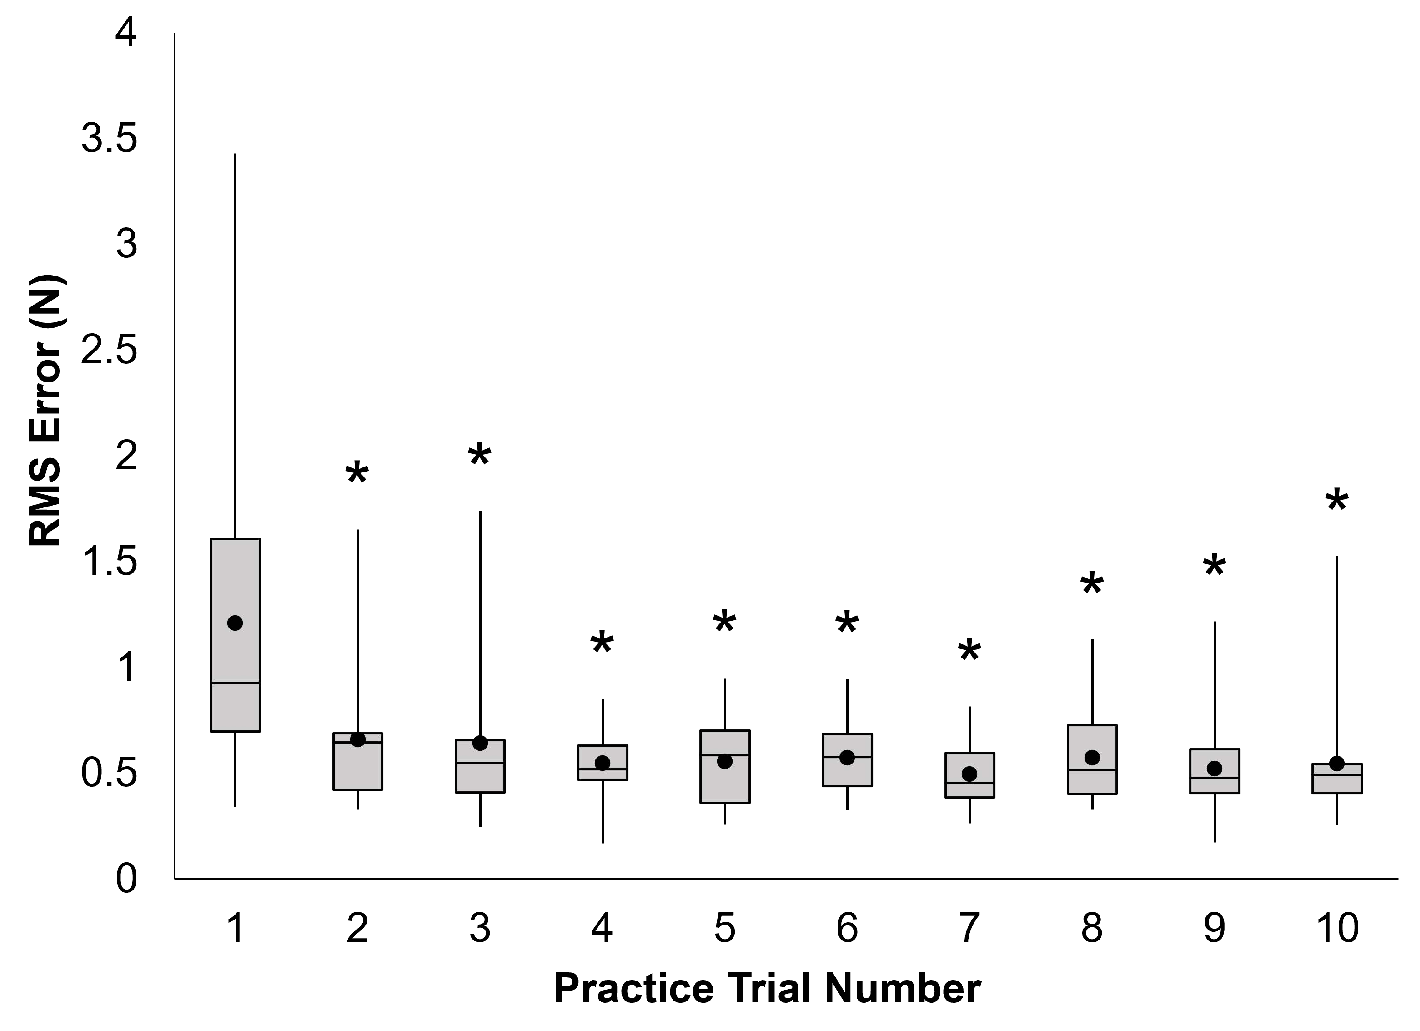
\includegraphics[width=1\textwidth,height=\textheight]{./figures/fig2.pdf}

}

\caption{\label{fig-2}Box plots presenting 1st quartile, median, and 3rd
quartile force stabilization RMS errors for each practice trial attempt.
Top and bottom whiskers present the max and min RMS errors,
respectively. The dots indicate the mean RMS error for each stimulation
level. The symbol * indicates a significant difference (p \textless{}
0.001) between mean RMS error during that practice trial compared to the
first trial.}

\end{figure}

To further investigate practice performance, the best practice trial was
identified for each subject, and the remaining trials were identified as
``best-i'' or ``best+i'' where ``i'' preserved the sequence in which
they were collected relative to the best trial. For example, if a
subject's best performance was recorded for their fourth practice trial,
this trial was identified as ``best''. Practice trials 1-3 were labeled
best-3, best-2, best-1, and trials following the best performance were
labeled as best+1, best+2, etc. Using a linear mixed model with trial as
a within-subjects factor and subject as a random effect, RMS error was
compared between different trial levels. Post-hoc planned comparisons
revealed significant differences (ranging from t(145) = -3.14, p = 0.035
to t(146) = -6.56, p \textless{} 0.0001) between the best practice trial
and trials identified as best-9, best-8, best-7, and best-5. These
results indicate that the trials following the first 5 practice trials
best identify a performance plateau. Per these results, a subset of
practice trials 6-10 or 6-11 where applicable were identified as the
trials describing plateaued task performance during practice. This
plateau subset would be used in subsequent analyses to draw comparisons
to the stimulation trials.

\hypertarget{analyses-of-stimulation-trials}{%
\subsection{Analyses of Stimulation
Trials}\label{analyses-of-stimulation-trials}}

Group-level analyses of force stabilization RMS errors were first
evaluated by comparing performance at each stimulation level.
Performance at each stimulation level varied greatly between
participants (Figure~\ref{fig-3}). Multilevel model analyses were
conducted with stimulation level as a fixed effect and subject as random
intercept effect. No differences were observed between the RMS errors
for the stimulation levels or the pre- or post-sham trials (F(11,187) =
1.45, p = .15). The largest RMS error magnitude (0.54 N) and standard
error (0.084 N), however, occurred for the final sham trial (post-sham)
following the completion of noise stimulation trials. To examine whether
this increase is due to a fatigue effect, a Pearson correlation was
calculated between RMS error and the sequential trial number. No
fatigue-related time-on-task effects were found (r(16) = .12, p
\textgreater{} .6).

\begin{figure}

{\centering 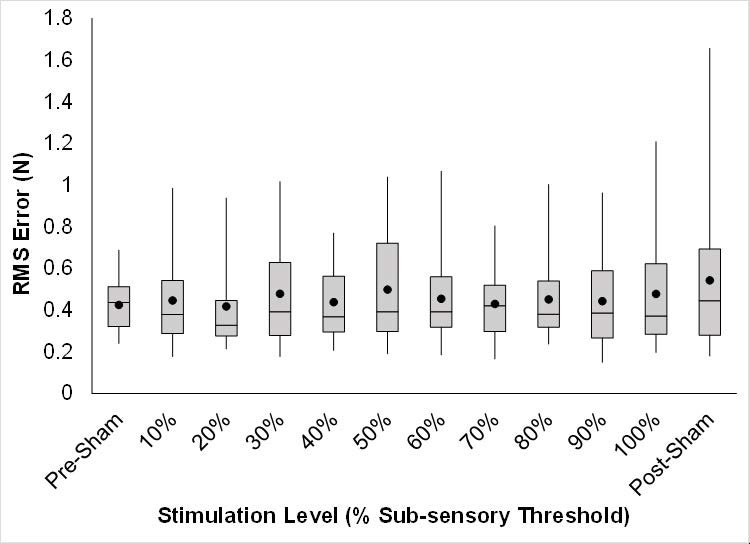
\includegraphics[width=1\textwidth,height=\textheight]{./figures/fig3.pdf}

}

\caption{\label{fig-3}Box plots presenting 1st quartile, median, and 3rd
quartile force stabilization RMS errors for each stimulation level. Top
and bottom whiskers present the max and min RMS errors, respectively,
for each stimulation level. The dots indicate the mean RMS error for
each stimulation level.}

\end{figure}

To determine whether performance during stim trials differed from
performance during practice, the RMS errors for the practice plateau
subset were compared to the RMS errors during all stimulation trials. A
one-way ANOVA analysis was completed with trial type as a
within-subjects effect (two levels = practice, stim) and subject as a
random effect. A log transform was used to satisfy the normality
assumption, and results indicated no statistically significant
difference (F(1,17) = 1.189, p = 0.291) between the mean RMS error
during practice (0.54±0.17 N) and during all stim trials (0.49±0.13 N).

While the mean performance for all stim trials did not differ from
practice performance, the primary interest of this study was whether
individualized principal noise stim would result in improved
performance. An individual's principal noise stimulation level was
assigned as the noise stimulation trial for which they exhibited the
best force stabilization performance (lowest RMS error).
Figure~\ref{fig-4} presents the RMS errors recorded for a single
participant exhibiting principal stimulation at 30\% sub-sensory
threshold.

One-way ANOVA analyses were repeated comparing RMS errors between the
plateau subset and the performance during individual principal noise
stimulation. A significant main effect of trial type was found (F(1,16)
= 26.313, p = 0.0001, d = 0.41). RMS error during principal noise
stimulation (0.35±0.11 N) was significantly less than the RMS error
during practice trials (0.54±0.17 N).

Principal stimulation levels varied widely across the group such that
each sub-sensory stimulation level was found to be the principal
stimulation level for at least one participant. To further examine the
relationship between RMS errors and stimulation level for the group, the
data was restructured such that the RMS error corresponding to an
individual's principal stimulation level was assigned the label ``prin
noise'', and their RMS errors associated with the remaining stimulation
trials were labeled as a positive or negative percent difference
(\%diff) from the individual's principal stimulation level. For example,
for the data presented in Figure~\ref{fig-4}, the error at 30\%
sub-sensory threshold was identified as ``prin noise'', and the errors
at 10, 20, 40, and 50\% were identified as 20, 10, +10, and +20 \%diff,
respectively, from the principal stimulation level. Once RMS errors for
all participants were relabeled using this convention, the errors were
averaged for the principal stimulation level and for each \%diff
stimulation level (Figure~\ref{fig-5}). The result of this data
presentation is that the number of values contributing to the mean and
error calculations are different between stimulation levels.

\begin{figure}

{\centering 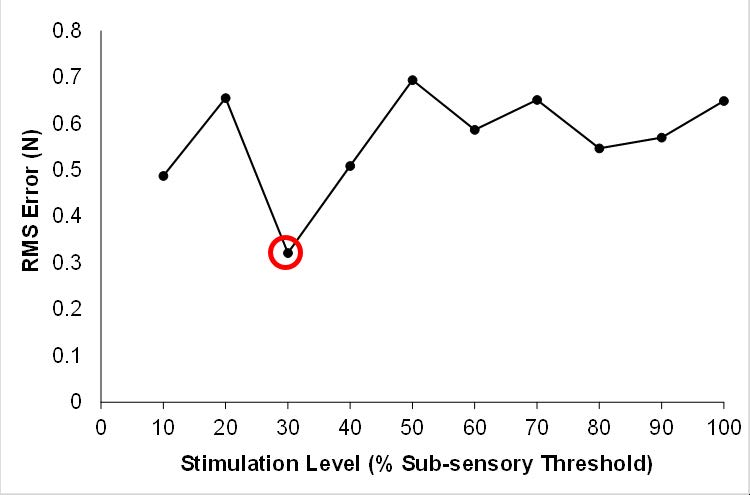
\includegraphics{./figures/fig4.pdf}

}

\caption{\label{fig-4}RMS errors for a single participant at each
stimulation level. Principal stimulation level was identified at 30\%
and is indicated by the circled data point.}

\end{figure}

\begin{figure}

{\centering 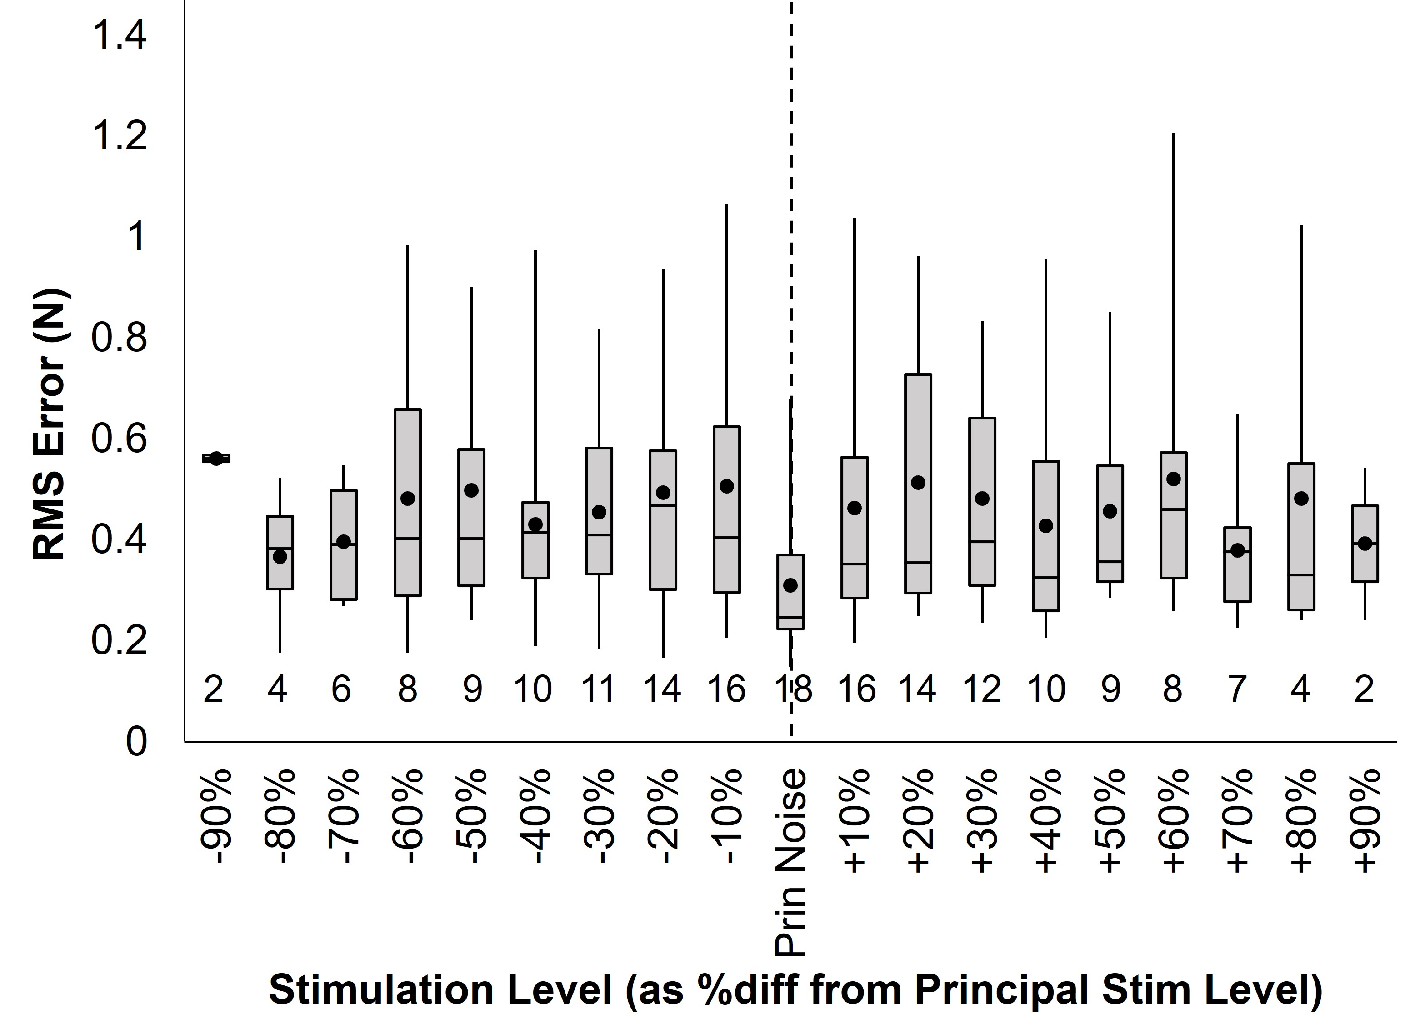
\includegraphics{./figures/fig5.pdf}

}

\caption{\label{fig-5}Box plots presenting 1st quartile, median, and 3rd
quartile RMS errors for each stimulation level. Top and bottom whiskers
present the maximum and minimum RMS errors for each level, respectively.
The dots indicate the mean RMS error for each stimulation level. The
number of observations used to determine mean, quartiles, maximum, and
minimum values are provided as sample size corresponding to each
stimulation level.}

\end{figure}

Group-level analysis was then conducted to determine if performance at
the principal stimulation level was significantly better than
performance at other stimulation levels expressed as \%diff from this
principal level. Model estimated marginal means, standard error, and
confidence intervals are provided for each stimulation level in
Table~\ref{tbl-1}. When examining the RMS errors as a function of \%diff
from principal stimulation, the best performance as a group was observed
at the principal stimulation level. Multilevel analyses revealed that
the model estimate RMS error recorded for the principal stimulation
level was significantly different (F(18,145) = 3.06, p \textless{}
.0001) than the RMS errors for a number of stimulation levels using
Dunnett's test (Dunnett, 1955) to correct for multiple comparisons. For
stimulation levels ranging from -60\% to +60\%, all but the -30\% level
had t scores ranging from 3.28 ≤ t(145) ≤ 5.46 and significance levels
of p ≤ .019 (d = 0.71 to 1.04). The stimulation level of -30\% fell just
outside the cutoff for significance with t(145) = 2.92, p = .053.
Estimated RMS errors at stimulation levels of -90\% and +80\% were also
significantly different than mean RMS error at the principal stimulation
level (t(145) = 3.08, p = .035, d = 1.85 and t(145) = 3.61, p = .007, d
= 0.89, respectively). In addition to the differences in estimated RMS
values, the variation in performance as indicated by the box plot sizes
also suggests that RMS errors at the principal stimulation level had a
narrower distribution than errors recorded for other stimulation levels.
To further validate this principal noise stimulation level, an identical
analysis was performed on the errors measured during the practice
trials. When completing the same ANOVA and post-hoc analyses on the
ordered practice trial errors, the performance during the best practice
trial was only significantly better than the first five attempts (t(146)
= -6.57 to t(145) = -3.14, p = \textless0.0001 to 0.035, d = 2.46 to
0.92). This lent further support to the identification of the principal
noise level as a special case.

\hypertarget{tbl-1}{}
\begin{table}
\caption{\label{tbl-1}Estimated marginal means, standard errors, and 95\% confidence intervals
(CI) from the multilevel statistical model. }\tabularnewline

\centering
\begin{tabular}[t]{c>{\centering\arraybackslash}p{2cm}>{\centering\arraybackslash}p{2cm}>{\centering\arraybackslash}p{2cm}>{\centering\arraybackslash}p{2cm}>{\centering\arraybackslash}p{2cm}}
\toprule
Stimulation Level & Estimated Marginal Mean (N) & Standard Error (N) & df & Lower 95\% CI & Upper 95\% CI\\
\midrule
-90\% & 0.5475 & 0.0882 & 109.15 & 0.3726 & 0.7224\\
-80\% & 0.4177 & 0.0714 & 64.09 & 0.2751 & 0.5603\\
-70\% & 0.4352 & 0.0647 & 46.49 & 0.3050 & 0.5654\\
-60\% & 0.4586 & 0.0610 & 37.81 & 0.3351 & 0.5822\\
-50\% & 0.4850 & 0.0597 & 34.96 & 0.3638 & 0.6063\\
\addlinespace
-40\% & 0.4410 & 0.0586 & 32.68 & 0.3217 & 0.5603\\
-30\% & 0.4229 & 0.0577 & 30.83 & 0.3051 & 0.5406\\
-20\% & 0.4844 & 0.0557 & 27.02 & 0.3701 & 0.5988\\
-10\% & 0.4955 & 0.0548 & 25.37 & 0.3828 & 0.6084\\
Prin Noise & 0.3106 & 0.0541 & 24.14 & 0.1989 & 0.4222\\
\addlinespace
+10\% & 0.4653 & 0.0548 & 25.37 & 0.3525 & 0.5781\\
+20\% & 0.4992 & 0.0557 & 27.02 & 0.3849 & 0.6136\\
+30\% & 0.4634 & 0.0569 & 29.32 & 0.3470 & 0.5798\\
+40\% & 0.4467 & 0.0586 & 32.67 & 0.3274 & 0.5660\\
+50\% & 0.4706 & 0.0597 & 34.96 & 0.3493 & 0.5918\\
\addlinespace
+60\% & 0.5083 & 0.0610 & 37.82 & 0.3847 & 0.6318\\
+70\% & 0.4309 & 0.0626 & 41.50 & 0.3045 & 0.5773\\
+80\% & 0.5160 & 0.0713 & 63.98 & 0.3735 & 0.6585\\
+90\% & 0.4831 & 0.0882 & 109.07 & 0.3082 & 0.6579\\
\bottomrule
\end{tabular}
\end{table}

\begin{figure}

{\centering 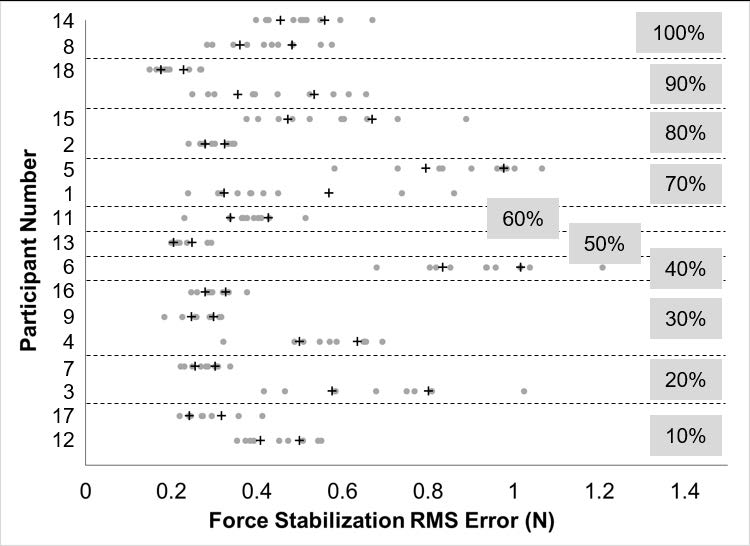
\includegraphics[width=1\textwidth,height=\textheight]{./figures/fig6.pdf}

}

\caption{\label{fig-6}RMS errors recorded for each of 10 stimulation
levels. The symbol ``+'' for each data set indicates the upper and lower
limits of the 95\% confidence interval. Individual subject data is
presented and grouped by principal stimulation level. Shaded values on
the right indicate the principal stimulation level as a percent of
individual sub-sensory threshold.}

\end{figure}

Individual one-sided Dixon Q tests were conducted to determine whether
the minimum RMS error recorded for a given participant could be
identified as significantly different from the group of RMS errors
recorded for other stimulation levels. Two participants (participants 4
and 11) demonstrated RMS errors that were significantly lower (Q = .50,
p = .039 and Q = .54, p = .024, respectively) than the remaining
distribution of errors recorded for the other stimulation levels. To
further inspect the distribution of errors for each participant,
parametric 95\% confidence intervals were calculated for each individual
(Figure~\ref{fig-6}). The difference between a participant's lowest RMS
error and their lower 95\% confidence limit ranged from 0.005 N -- 0.21
N with a group mean difference of 0.08±0.06 N. As stated previously, no
consistency was observed in the sub-sensory stimulation level eliciting
the best force stabilization (Figure~\ref{fig-6}). Among the 18
participants, each sub-sensory stimulation level was found to be the
principal level for at least one individual (Figure~\ref{fig-6}).

Following the force stabilization trials, the input voltages identified
as the mean principal noise stimulation level had a range of 0.005-0.16
V with a group mean of 0.06±0.05 V. This mean principal stimulation
voltage corresponded to acceleration magnitudes of 0.035-0.15 G across
the frequency spectrum of the stimulation signals. To examine whether
significant relationships exist between threshold, principal stimulation
level, and MVC values, Spearman correlations were calculated for each
pair of measures. Spearman, rather than Pearson, correlations were used
due to the lack of normality for the threshold and principal stimulation
level measures as determined by the Shapiro-Wilk test (W = .80, p = .002
and W = .83, p = .005, respectively). Moderate but significant Spearman
correlations were observed between threshold and MVC (rs = .49, p =
.041) and principal stimulation level and MVC (rs = .56, p = .016).
Increases in MVC are associated with increases in both threshold and
principal stimulation level. A strong significant Spearman correlation
was observed between threshold level and principal stimulation level (rs
= .65, p = .003).

\hypertarget{discussion}{%
\section{Discussion}\label{discussion}}

The MVC measures recorded for most (n=15) participants were largely
similar in magnitude to the maximum isometric finger forces reported by
Cort \& Potvin (\protect\hyperlink{ref-cort2011}{2011}). The lower (32.2
N) and upper bounds (168.7 N and 188.2 N), however, were somewhat
extreme for single finger flexion. In both instances, the experimental
apparatus may account for these variations. Our setup required
participants to grip the trigger mechanism with the middle phalanx of
the second finger, and the trigger was custom printed using a rigid
thermoplastic. While a more proximal application site is reported to
increase maximum isometric finger force
(\protect\hyperlink{ref-cort2011}{Cort \& Potvin, 2011}), the contact
between the finger and trigger could be uncomfortable to some. It's
likely that the perceived discomfort of the apparatus may have limited a
participant's MVC. Alternatively, other participants may have found it
difficult to isolate the finger flexor exertion and involved other
muscles (i.e.~biceps). While their MVCs may be extreme, these
participants were retained in the data set because they otherwise met
the requirement for MVC determination. In each case, the MVC was a
consistent and reproducible value for the participant under our
experimental conditions, and they were able to complete the
ramp-and-hold trials reliably.

It is also worth acknowledging here that the stimulation in this study
was applied to the wrist rather than at the point of force application.
This choice was made in support of a larger motor control study
(\protect\hyperlink{ref-Tenan2019}{Tenan et al., 2019}) that followed
the stimulation selection presented here. In that study, participants
completed a series of force stability tasks during which motor unit
firing, electroencephalography, and reflex response data were recorded.
The stimulation was applied at the wrist to stimulate muscle spindle
receptors and to ensure that the stimulation was part of the
afferent/efferent feedback loop of the flexor digitorum muscle
controlling the finger. Results suggested that behavioral changes
observed during vibrotactile stimulation are likely due to tonic
vibration reflex in the muscle tendons
(\protect\hyperlink{ref-Tenan2019}{Tenan et al., 2019}).

In general, group level performance of a finger force stability task was
significantly improved when participants received stimulation
corresponding to their individually identified principal stimulation
level. When performance was assessed at an individual level, however,
RMS errors during principal stimulation trials were only significantly
different from the distribution of errors across other noise stimulation
trials for 2 participants. Principal stimulation levels were shown to be
highly variable, and this study suggests that the performance
improvement compared with other levels of stimulation were marginal for
most individuals. In fact, when comparing all stim trials to the
practice plateau, significant differences in performance were not
observed. Performance at the principal noise stimulation level showed
improvement at the group level but may in fact provide only marginal
improvement over performance during other stim levels.

Despite a broad range in MVC measures and sub-sensory thresholds (0.02
to 0.35V), half of the participants (9 of 18) exhibited their
sub-sensory threshold level at 0.05 V. The reason for the cluster of
threshold levels at 0.05 V, however, is unclear. Noise signals were
evaluated for threshold in increments of 0.05 V. The next highest noise
magnitude was 0.10 V. It may be that the acceleration magnitudes
imparted by the stimulator between input voltages of 0.10 and 0.05 V are
very near the central distribution of perception. The 0.05 V step
between these two input voltages may have been too coarse to
specifically pinpoint the input voltage level at which sensation ceases.
Future studies may utilize finer steps between input voltages to
identify sub-sensory threshold levels.

Individual performance during the finger flexion force stability task
with a specific noise stimulation level varied substantially. The
variability was so large that, when averaged among all participants, the
presence of any group-level principal stimulation level was obscured.
Similar findings were reported by Manjarrez et al.
(\protect\hyperlink{ref-Manjarrez2002}{2002}) who noted considerable
variability in the shape of electroencephalography signal-to-noise ratio
profiles obtained for different participants receiving the same input
noise levels. Individual responses to noise stimulation appear to be
highly variable and are not easily or effectively described via standard
summary statistics. Mulavara et al.
(\protect\hyperlink{ref-Mulavara2015}{2015}) also found similar results
with electrical vestibular stimulation. Although they reported a group
average optimal stimulation level equivalent to 35\% of perceptual
threshold, individuals exhibited optimal stimulation levels ranging from
8-100\% of perceptual threshold. Additionally, using electrical
vestibular stimulation, Goel et al.
(\protect\hyperlink{ref-Goel2015}{2015}) reported that during each of 4
studies, only a subset of participants were considered ``responsive'' to
stimulation. Large inter-subject variability and the existence of
``non-responders'' to stimulation make the study of optimal noise
stimulation levels challenging. Of note in the present study, however,
is that the largest RMS error and largest variability occurred for the
final sham trial. This suggests that noise stimulation, regardless of
its level, may have imparted some degree of stabilization in the
preceding trials, and its absence during the final sham trial may have
resulted in poorer performance across participants. This finding raises
a concern not often addressed in the noise stimulation literature. It
may be relevant to quantify the effects of noise stimulation cessation.

Two different attempts were made to determine if the principal level of
stimulation improved stability. The first analysis performed a partial
pooling of all subject's data using a multilevel model with the data
restructured and centered at each individual's principal stimulation
level. This analysis revealed that there did appear to be a statistical
difference between the level of stimulation eliciting the greatest
stability and other levels of stimulation. These results support
previous research indicating that specific noise levels can enhance
motor performance (\protect\hyperlink{ref-Manjarrez2002}{Manjarrez et
al., 2002}; \protect\hyperlink{ref-Mendez-Balbuena2012}{Mendez-Balbuena
et al., 2012}). The second analysis considered individual subject data
and attempted to determine if the behavioral outcome (i.e., RMS error)
from the principal stimulation level was a statistical outlier compared
to all other trials. These results failed to show that the principal
stimulation level was an outlying case for most subjects. For only two
participants was the RMS error during their principal noise trial
significantly lower than the error during other trials. For these
individuals, principal stimulation level appears to have produced better
motor performance. It is noted, however, that principal stimulation
levels resulted in force stabilization RMS errors which fell outside the
95\% CI for all subjects. It is possible that not enough data points
were collected to effectively determine if stability during the
principal stimulation level resides outside the expected performance
distribution of at other stimulation levels. Future research in this
area should obtain data at more points along the continuum of
stimulation or perform repeated testing on the same stimulation levels
to confirm the selection of a principal or optimal noise level.

As reported previously (\protect\hyperlink{ref-Manjarrez2002}{Manjarrez
et al., 2002};
\protect\hyperlink{ref-Mendez-Balbuena2012}{Mendez-Balbuena et al.,
2012}), the best performance stimulation level for individuals varied
widely, and RMS error curves exhibited a variety of shapes. Manjarrez et
al. (\protect\hyperlink{ref-Manjarrez2002}{2002}) arbitrarily defined 3
bands of noise and classified their participants as responders to either
low, intermediate, or high levels of noise stimulation. The majority of
their participants exhibited optimal performance within the high range
of noise stimulation. Using the same technique, we would define our low,
intermediate, and high noise levels as bands consisting of 10-30\%,
40-70\%, and 80-100\%, respectively. Principal noise in our study,
however, was more evenly distributed among the three identified bands of
noise with 7 participants exhibiting principal noise stimulation in the
low band, 5 in the intermediate band, and the remaining 6 in the high
band. Currently, research employing vibratory noise stimulation often
applies noise at a specific percentage (\textasciitilde70-90\%) of
sub-sensory threshold level (\protect\hyperlink{ref-Galica2009}{Galica
et al., 2009}; \protect\hyperlink{ref-Lipsitz2015}{Lipsitz et al.,
2015}; \protect\hyperlink{ref-Priplata2002}{A. Priplata et al., 2002}).
Results from these studies clearly indicate that this arbitrary noise
level does elicit a stabilizing effect compared to no stimulation.
However, this commonly used stimulation level may actually only be
eliciting the optimal stabilization effects for about 1/3 of the
participants. Greater stabilization may be possible if optimal
stimulation levels can be identified and applied; however, this level of
customization may be unnecessary in some motor tasks or provide only
marginal benefits over an arbitrary stimulation level.

Studies using designs similar to ours have indicated that an optimal
level of noise is required to obtain a maximal effect of noise
stimulation (\protect\hyperlink{ref-Manjarrez2002}{Manjarrez et al.,
2002}; \protect\hyperlink{ref-Mendez-Balbuena2012}{Mendez-Balbuena et
al., 2012}; \protect\hyperlink{ref-Trenado2014}{Trenado et al., 2014}).
Our results, however, do not exhibit a robust optimal noise phenomenon
with a predictable inverted-U pattern. While the optimal noise pattern
is a classical hallmark of stochastic resonance within a non-linear
system, the present study focused on two different systems: the
somatosensory and the motor systems. It is possible that the SR-like
benefit in the somatosensory system does not translate directly into the
motor system, which is receiving numerous neurological inputs to
generate force. The two previous study designs showing an inverted-U
optimal noise pattern were also focused on fingertip displacement
(\protect\hyperlink{ref-Manjarrez2002}{Manjarrez et al., 2002};
\protect\hyperlink{ref-Mendez-Balbuena2012}{Mendez-Balbuena et al.,
2012}). It is possible that some characteristics of noise stimulation on
motor behavior are only able to be differentiated within specific
paradigms and not widely generalizable to other tasks.

As a final quantitative analysis of the present data, Spearman
correlation coefficients were calculated for MVC, sub-sensory
stimulation thresholds, and optimal noise stimulation level. Spearman
correlations determine how well the rank order of one variable
corresponds to the rank order of another. Strong correlations indicate
that as the rank of one variable increases, the rank of the other
responds in a predictable way following a linear or non-linear function.
Significant moderate to strong correlations were found suggesting that a
higher MVC and a higher sub-sensory threshold level are associated with
higher principal stimulation levels. A larger MVC was also associated
with a higher sensory threshold. These relationships are relevant when
customizing stimulation. Individuals with a larger MVC magnitude likely
warrant a greater stimulation magnitude for customized noise
stimulation. However, the quantitative relationship between principal
noise stimulation, sub-sensory threshold level, and finger flexion MVC
was not identified here. Simplifying the selection of principal noise
stimulation level would expedite its use in research and in clinical
applications. More research is needed to determine if in fact an optimal
stimulation level is essential for clinical interventions and, if so,
whether an individual's optimal stimulation level may be effectively
identified via a more easily quantified measure such as strength or
perceptual threshold.

\hypertarget{limitations}{%
\section{Limitations}\label{limitations}}

A primary limitation of this study was the completion of only a single
trial for each noise stimulation level. While other studies have been
conducted in a similar fashion
(\protect\hyperlink{ref-Manjarrez2002}{Manjarrez et al., 2002};
\protect\hyperlink{ref-Mendez-Balbuena2012}{Mendez-Balbuena et al.,
2012}; \protect\hyperlink{ref-Trenado2014}{Trenado et al., 2014}),
collecting additional trials would have provided a measure of
performance variability for each noise level and afforded reliability
analyses for the principal stimulation level. Additionally, there is
some uncertainty regarding the duration of the effects of stimulation.
For this study, participants received a particular level of stimulation
for the duration of a given trial. It is unclear whether exposure time
to imperceptible stimulation has an influence on its behavioral effects.
Lastly, sensory threshold was quantified using scaled white Gaussian
noise transmitted through the stimulator. While this enabled a direct
translation between the measurement of sensory threshold and the
application of desired subsensory noise, this study may have benefitted
from the use of the Semmes-Weinstein monofilament test to provide a more
standardized measure of tactile sensitivity. Such a measure could have
identified the sensory threshold with greater accuracy and resolution
than the approach employed here and allowed for more customized
subsensory stimulation.

\hypertarget{conclusions}{%
\section{Conclusions}\label{conclusions}}

Despite tightly controlling other signal properties and varying only
noise amplitude, the principal stimulation level varied considerably
between individuals. At the group level, vibrotactile stimulation
applied at a customized principal noise level resulted in better force
stabilization performance compared to practice trials and other
stimulation levels. At the individual level, however, outlier analyses
failed to report significant differences in individual performance at
the principal stimulation level compared to the remaining trials. This
may indicate that, while principal stimulation provides the best
performance, its benefits may only marginally outweigh noise stimulation
at an arbitrary imperceptible level when focusing on fingertip
displacement. Additional work is needed to determine the reliability of
the principal noise stimulation levels identified using this procedure.
Further, this work focuses on a simple, controlled fine motor task, and
these results may not apply to more dynamic or whole-body physical
tasks. More work is needed is explore physical task performance during
exposure to varied levels of vibrotactile stimulation and to determine
the best implementation of vibrotactile noise for stability or assistive
devices.

\newpage

\hypertarget{additional-information}{%
\section{Additional Information}\label{additional-information}}

\hypertarget{data-accessibility}{%
\subsection{Data Accessibility}\label{data-accessibility}}

All data and analysis code used for this manuscript are available at
\url{https://osf.io/cah3j}.

\hypertarget{author-contributions}{%
\subsection{Author Contributions}\label{author-contributions}}

Courtney A. Haynes contributed to this work as a co-investigator
assisting with the design the experimental paradigm, developing custom
data collection programs, pilot testing procedures, and executing the
data collection. Dr.~Haynes completed the analyses described in this
paper and led the writing of the various manuscript drafts incorporating
revisions provided by her co-authors. Dr.~Haynes consents to the
publication of this manuscript in its present form.

Matthew S. Tenan contributed to this work as a principal investigator
leading the design of the experimental paradigm and executing the full
data collection. Dr.~Tenan has contributed substantially to the content
by providing thorough reviews of the manuscript, providing additional
content, and assisting with the interpretation of the study's findings.
Dr.~Tenan consents to the publication of this manuscript in its present
form.

Antony D. Passaro is a co-investigator for this work assisting with the
design of the experimental paradigm and providing his expertise
regarding data analysis techniques to examine the study results.
Dr.~Passaro also provided valuable suggestions for data presentation and
provided critical revisions for the manuscript drafts. Dr.~Passaro has
provided his consent for publication of this manuscript in its present
form.

Andrew J. Tweedell served as a co-investigator assisting with design of
the experiment, hardware acquisition and establishing the experimental
apparatus, pilot testing, and executing the data collection with human
subjects. Mr.~Tweedell has provided extensive manuscript revisions and
provided insights regarding data analysis and interpretation.
Mr.~Tweedell has provided his consent for publication of this manuscript
in its present form.

Contributed to conception and design: CAH, MST, ADP, AJT Contributed to
acquisition of data: CAH, MST, AJT Contributed to analysis and
interpretation of data: CAH, MST, ADP, AJT Draft and/or revised the
article: CAH, MST, ADP, AJT Approved the submitted version for
publication: CAH, MST, ADP, AJT

\hypertarget{conflict-of-interest}{%
\subsection{Conflict of Interest}\label{conflict-of-interest}}

The authors declare that this research was conducted independently and
free of any personal or financial relationships that could be construed
as a conflict of interest.

\hypertarget{funding}{%
\subsection{Funding}\label{funding}}

This work was funded by the Department of Defense Human Systems
Integration (Cybernetics) research line at the U.S. Army Research
Laboratory (74-A-HRCYB).

\hypertarget{acknowledgments}{%
\subsection{Acknowledgments}\label{acknowledgments}}

Many thanks to Mr.~Mike Kosinski and Mr.~Dave Kuhn for their hard work
designing and fabricating the instrumented grip apparatus and the arm
cradle used for data collection. Thanks also to Dr.~J. Cortney Bradford,
Mr.~Paul Riggs, and the facilities staff at the Army Research Laboratory
Mission Impact through Neuro-inspired Design (MIND) lab for the use of
their equipment and lab facilities.

\newpage

\hypertarget{references}{%
\section{References}\label{references}}

\hypertarget{refs}{}
\begin{CSLReferences}{1}{0}
\leavevmode\vadjust pre{\hypertarget{ref-benzi1981}{}}%
Benzi, R., Sutera, A., \& Vulpiani, A. (1981). The mechanism of
stochastic resonance. \emph{Journal of Physics A: Mathematical and
General}, \emph{14}(11), L453--L457.
\url{https://doi.org/10.1088/0305-4470/14/11/006}

\leavevmode\vadjust pre{\hypertarget{ref-Bezrukov1995}{}}%
Bezrukov, S. M., \& Vodyanoy, I. (1995). Noise-induced enhancement of
signal transduction across voltage-dependent ion channels.
\emph{Nature}, \emph{378}(6555), 362--364.
\url{https://doi.org/10.1038/378362a0}

\leavevmode\vadjust pre{\hypertarget{ref-Collins2003}{}}%
Collins, J. J., Priplata, A. A., Gravelle, D. C., Niemi, J., Harry, J.,
\& Lipsitz, L. A. (2003). Noise-enhanced human sensorimotor function.
\emph{IEEE Engineering in Medicine and Biology Magazine}, \emph{22}(2),
76--83. \url{https://doi.org/10.1109/memb.2003.1195700}

\leavevmode\vadjust pre{\hypertarget{ref-cort2011}{}}%
Cort, J. A., \& Potvin, J. R. (2011). Maximum isometric finger pull
forces. \emph{International Journal of Industrial Ergonomics},
\emph{41}(2), 91--95. \url{https://doi.org/10.1016/j.ergon.2010.12.008}

\leavevmode\vadjust pre{\hypertarget{ref-dunnett1955}{}}%
Dunnett, C. W. (1955). A Multiple Comparison Procedure for Comparing
Several Treatments with a Control. \emph{Journal of the American
Statistical Association}, \emph{50}(272), 1096--1121.
\url{https://doi.org/10.1080/01621459.1955.10501294}

\leavevmode\vadjust pre{\hypertarget{ref-Galica2009}{}}%
Galica, A. M., Kang, H. G., Priplata, A. A., D'Andrea, S. E.,
Starobinets, O. V., Sorond, F. A., Cupples, L. A., \& Lipsitz, L. A.
(2009). Subsensory vibrations to the feet reduce gait variability in
elderly fallers. \emph{Gait \& Posture}, \emph{30}(3), 383--387.
\url{https://doi.org/10.1016/j.gaitpost.2009.07.005}

\leavevmode\vadjust pre{\hypertarget{ref-gammaitoni1998}{}}%
Gammaitoni, L., Hänggi, P., Jung, P., \& Marchesoni, F. (1998).
Stochastic resonance. \emph{Reviews of Modern Physics}, \emph{70}(1),
223--287. \url{https://doi.org/10.1103/revmodphys.70.223}

\leavevmode\vadjust pre{\hypertarget{ref-Goel2015}{}}%
Goel, R., Kofman, I., Jeevarajan, J., De Dios, Y., Cohen, H. S.,
Bloomberg, J. J., \& Mulavara, A. P. (2015). Using Low Levels of
Stochastic Vestibular Stimulation to Improve Balance Function.
\emph{PLOS ONE}, \emph{10}(8), e0136335.
\url{https://doi.org/10.1371/journal.pone.0136335}

\leavevmode\vadjust pre{\hypertarget{ref-Lakshminarayanan2015}{}}%
Lakshminarayanan, K., Lauer, A. W., Ramakrishnan, V., Webster, J. G., \&
Seo, N. J. (2015). Application of vibration to wrist and hand skin
affects fingertip tactile sensation. \emph{Physiological Reports},
\emph{3}(7), e12465. \url{https://doi.org/10.14814/phy2.12465}

\leavevmode\vadjust pre{\hypertarget{ref-Lipsitz2015}{}}%
Lipsitz, L. A., Lough, M., Niemi, J., Travison, T., Howlett, H., \&
Manor, B. (2015). A Shoe Insole Delivering Subsensory Vibratory Noise
Improves Balance and Gait in Healthy Elderly People. \emph{Archives of
Physical Medicine and Rehabilitation}, \emph{96}(3), 432--439.
\url{https://doi.org/10.1016/j.apmr.2014.10.004}

\leavevmode\vadjust pre{\hypertarget{ref-magalhuxe3es2011}{}}%
Magalhães, F. H., \& Kohn, A. F. (2010). Vibratory noise to the
fingertip enhances balance improvement associated with light touch.
\emph{Experimental Brain Research}, \emph{209}(1), 139--151.
\url{https://doi.org/10.1007/s00221-010-2529-3}

\leavevmode\vadjust pre{\hypertarget{ref-Manjarrez2002}{}}%
Manjarrez, E., Diez-Martıńez, O., Méndez, I., \& Flores, A. (2002).
Stochastic resonance in human electroencephalographic activity elicited
by mechanical tactile stimuli. \emph{Neuroscience Letters},
\emph{324}(3), 213--216.
\url{https://doi.org/10.1016/s0304-3940(02)00212-4}

\leavevmode\vadjust pre{\hypertarget{ref-McDonnell2009}{}}%
McDonnell, M. D., \& Abbott, D. (2009). What Is Stochastic Resonance?
Definitions, Misconceptions, Debates, and Its Relevance to Biology.
\emph{PLoS Computational Biology}, \emph{5}(5), e1000348.
\url{https://doi.org/10.1371/journal.pcbi.1000348}

\leavevmode\vadjust pre{\hypertarget{ref-Mendez-Balbuena2012}{}}%
Mendez-Balbuena, I., Manjarrez, E., Schulte-Monting, J., Huethe, F.,
Tapia, J. A., Hepp-Reymond, M.-C., \& Kristeva, R. (2012). Improved
Sensorimotor Performance via Stochastic Resonance. \emph{Journal of
Neuroscience}, \emph{32}(36), 12612--12618.
\url{https://doi.org/10.1523/jneurosci.0680-12.2012}

\leavevmode\vadjust pre{\hypertarget{ref-Moss2004}{}}%
Moss, F. (2004). Stochastic resonance and sensory information
processing: a tutorial and review of application. \emph{Clinical
Neurophysiology}, \emph{115}(2), 267--281.
\url{https://doi.org/10.1016/j.clinph.2003.09.014}

\leavevmode\vadjust pre{\hypertarget{ref-Moss2003}{}}%
Moss, F., \& Milton, J. G. (2003). Balancing the unbalanced.
\emph{Nature}, \emph{425}(6961), 911--912.
\url{https://doi.org/10.1038/425911a}

\leavevmode\vadjust pre{\hypertarget{ref-Mulavara2015}{}}%
Mulavara, A. P., Kofman, I. S., De Dios, Y. E., Miller, C., Peters, B.
T., Goel, R., Galvan-Garza, R., \& Bloomberg, J. J. (2015). Using low
levels of stochastic vestibular stimulation to improve locomotor
stability. \emph{Frontiers in Systems Neuroscience}, \emph{9}.
\url{https://doi.org/10.3389/fnsys.2015.00117}

\leavevmode\vadjust pre{\hypertarget{ref-Peng2018}{}}%
Peng, Y.-L., Tenan, M. S., \& Griffin, L. (2018). Hip position and sex
differences in motor unit firing patterns of the vastus medialis and
vastus medialis oblique in healthy individuals. \emph{Journal of Applied
Physiology}, \emph{124}(6), 1438--1446.
\url{https://doi.org/10.1152/japplphysiol.00702.2017}

\leavevmode\vadjust pre{\hypertarget{ref-Hur2014}{}}%
Pilwon Hur, Yao-Hung Wan, \& Na Jin Seo. (2014). Investigating the role
of vibrotactile noise in early response to perturbation. \emph{IEEE
Transactions on Biomedical Engineering}, \emph{61}(6), 1628--1633.
\url{https://doi.org/10.1109/tbme.2013.2294672}

\leavevmode\vadjust pre{\hypertarget{ref-Priplata2006}{}}%
Priplata, A. A., Patritti, B. L., Niemi, J. B., Hughes, R., Gravelle, D.
C., Lipsitz, L. A., Veves, A., Stein, J., Bonato, P., \& Collins, J. J.
(2005). Noise-enhanced balance control in patients with diabetes and
patients with stroke. \emph{Annals of Neurology}, \emph{59}(1), 4--12.
\url{https://doi.org/10.1002/ana.20670}

\leavevmode\vadjust pre{\hypertarget{ref-Priplata2002}{}}%
Priplata, A., Niemi, J., Salen, M., Harry, J., Lipsitz, L. A., \&
Collins, J. J. (2002). Noise-Enhanced Human Balance Control.
\emph{Physical Review Letters}, \emph{89}(23).
\url{https://doi.org/10.1103/physrevlett.89.238101}

\leavevmode\vadjust pre{\hypertarget{ref-purves2001}{}}%
Purves, D., Augustine, G. J., Fitzpatrick, D., Katz, L. C., LaMantia,
A.-S., McNamara, J. O., \& Williams, S. M. (2001). Mechanoreceptors
Specialized to Receive Tactile Information. \emph{Neuroscience. 2nd
Edition}. \url{https://www.ncbi.nlm.nih.gov/books/NBK10895/}

\leavevmode\vadjust pre{\hypertarget{ref-Simeonov2011}{}}%
Simeonov, P., Hsiao, H., Powers, J., Ammons, D., Kau, T., \& Amendola,
A. (2011). Postural stability effects of random vibration at the feet of
construction workers in simulated elevation. \emph{Applied Ergonomics},
\emph{42}(5), 672--681.
\url{https://doi.org/10.1016/j.apergo.2010.10.002}

\leavevmode\vadjust pre{\hypertarget{ref-Tenan2016}{}}%
Tenan, M. S., Hackney, A. C., \& Griffin, L. (2015). Maximal force and
tremor changes across the menstrual cycle. \emph{European Journal of
Applied Physiology}, \emph{116}(1), 153--160.
\url{https://doi.org/10.1007/s00421-015-3258-x}

\leavevmode\vadjust pre{\hypertarget{ref-Tenan2019}{}}%
Tenan, M. S., Tweedell, A. J., Haynes, C. A., \& Passaro, A. D. (2019).
The effect of imperceptible Gaussian tendon vibration on the Hoffmann
reflex. \emph{Neuroscience Letters}, \emph{706}, 123--127.
\url{https://doi.org/10.1016/j.neulet.2019.05.018}

\leavevmode\vadjust pre{\hypertarget{ref-Trenado2014}{}}%
Trenado, C., Mikulić, A., Manjarrez, E., Mendez-Balbuena, I.,
Schulte-Mönting, J., Huethe, F., Hepp-Reymond, M.-C., \& Kristeva, R.
(2014). Broad-band gaussian noise is most effective in improving motor
performance and is most pleasant. \emph{Frontiers in Human
Neuroscience}, \emph{8}. \url{https://doi.org/10.3389/fnhum.2014.00022}

\end{CSLReferences}



\end{document}
